\documentclass[aspectratio=169,xcolor=table]{beamer}
%aspcetratio >> 1610 169 149 54 43 32
%The themes:
%\usetheme[style=classic]{mharvellous}
%\usetheme[style=dark]{mharvellous}
%\usetheme[style=mracula]{mharvellous}
\usetheme[style=default]{mharvellous}
%*--------------------------------------------------
%\usepackage{helvet}
%*--------------------------------------------------
\usepackage{bibunits}  
%\setbeamertemplate{bibliography item}{[\theenumiv]}
\setbeamertemplate{bibliography item}{\insertbiblabel}
\defaultbibliography{bibliography}
%\defaultbibliographystyle{IEEEtran}
%\defaultbibliographystyle{amsalpha}
\defaultbibliographystyle{abntex2-alf}
%\bibliography{bibliography}
%\usepackage[backend=biber,style=alphabetic,citestyle=authoryear]{biblatex}
% \addbibresource{bibliography.bib}
%\usepackage{natbib}
\usepackage{bibentry}
%*--------------------------------------------------
\usepackage{lipsum}
\usepackage{epigraph}
\usepackage{graphicx}
\usepackage{multirow}
%\usepackage{enumitem}
\usepackage{array}
%\usepackage{multimedia}
\usepackage{media9}
%\usepackage{pdfpc-movie}
\usepackage{circledsteps}
\usepackage{listings}
\usepackage[normalem]{ulem}
%\usepackage{Sweave}
%\usepackage{xkeyval}
%\usepackage{palatino}
%\usepackage{pgfpages}
\usepackage{float}
%*--------------------------------------------------
\usepackage[timeinterval=1]{tdclock}
%\usepackage[font=Times,timeinterval=1, timeduration=200,resetatpages=all]{tdclock}
%\usepackage[font=Times,timeinterval=10, timeduration=2.0, timedeath=0, fillcolorwarningsecond=white!60!yellow,timewarningfirst=50,timewarningsecond=80,resetatpages=2]{tdclock}
%*--------------------------------------------------
\usepackage{url}
\usepackage{tabularx,booktabs}
\usepackage{threeparttable}
\usepackage[absolute, overlay]{textpos}
%*--------------------------------------------------
\usepackage{framed, color}
\usepackage[tikz]{bclogo}
\usepackage{spot}
\setspotlightcolor{red!50}
% %\setspotlightstyle{star, fill=red!50}
% %\setspotlightstyle{star points=7}
\usepackage{color,soul}
%\usepackage{xcolor}
\usepackage{tcolorbox}
\usepackage{xcolor}
\usepackage[export]{adjustbox}
\usepackage{verbatim}
\usetikzlibrary{trees,shapes,arrows}
\usepackage{fancyvrb}
\usepackage{float}
%*--------------------------------------------------
\usepackage{amsmath}
\usepackage{xfrac}
\usepackage{units}
\usepackage{ulem}
%*-------------------------------------------------------------------------------
%\newcolumntype{C}[1]{>{\centering\arraybackslash}m{#1}}
\newcolumntype{L}[1]{>{\raggedright\let\newline\\\arraybackslash\hspace{0pt}}m{#1}}
\newcolumntype{C}[1]{>{\centering\let\newline\\\arraybackslash\hspace{0pt}}m{#1}}
\newcolumntype{R}[1]{>{\raggedleft\let\newline\\\arraybackslash\hspace{0pt}}m{#1}}
%*-------------------------------------------------------------------------------
%\pgfpagesuselayout{2 on 1}[a4paper,border shrink=5mm]
%\setbeamertemplate{note page}[plain]
%\setbeameroption{show notes on second screen=bottom}
%*-------------------------------------------------------------------------------
\setbeameroption{hide notes}
%\setbeameroption{show only notes}
%\setbeameroption{show notes on second screen=right}
\setbeamertemplate{note page}{\pagecolor{yellow!5}\insertnote}
%*-------------------------------------------------------------------------------

%*-------------------------------------------------------------------------------
\title              {Título}
\subtitle           {Subtítulo}
\author             {Nome Sobrenome}
\email              {nome@site.com}
\advisor            {Orientador: Marco A. dos Reis}
\institute          {Robótica e Sistemas Autônomos, Senai Cimatec}
\date               {Mês de 202x}
% \ulogo        		{Template/logosenaicimatecnegativo}
% \ulogof             {Template/logosenaicimatec2020}
% \ulogoo        		{Template/rosa-logo}
% \ulistelement    	{Template/bullet-white}

%*-------------------------------------------------------------------------------
\graphicspath{{Source/pictures/}}
%*-------------------------------------------------------------------------------
\totalNoSlidesDisabled % To turn off the total number of slides in the footer. Comment this if you want the total number of slides in the footer
%*-------------------------------------------------------------------------------
\begin{document}
%*----------- COVER -------------------------------------------------------------
 \begin{frame}[t,plain]
%*----------- sound--------------------------------
    \includemedia[
        %width=1ex,
        %height=1ex,
        %activate=pageopen, 
        activate=onclick,
        deactivate=onclick,
        %passcontext,
        transparent,
        addresource=./Source/sounds/hip-hop.mp3,
        flashvars={
                    source=./Source/sounds/hip-hop.mp3
                    %&autoPlay=true
                    &autoRewind=true
                    &Play=2s
                    &repeat=always
                    %&Loop=true
        }
    ]
    {}{VPlayer.swf}
%*----------- start-page--------------------------
    \titlepage
    %*----------- notes-------------------------------
    \note[item]{Notes can help you to remember important information. Turn on the notes option.}
\end{frame}
%-
%*----------- SECTIONS ----------------------------------------------------------
%*----------- SLIDE -------------------------------------------------------------
\begin{frame}[c]{Justificativa}
    \begin{itemize}
        \item acompanhamento, monitoramento e investigação subaquático
        \item dificuldade de acesso para mergulhadores
        \item regiões de riscos para os mergulhadores
    \end{itemize}

    \begin{figure}
        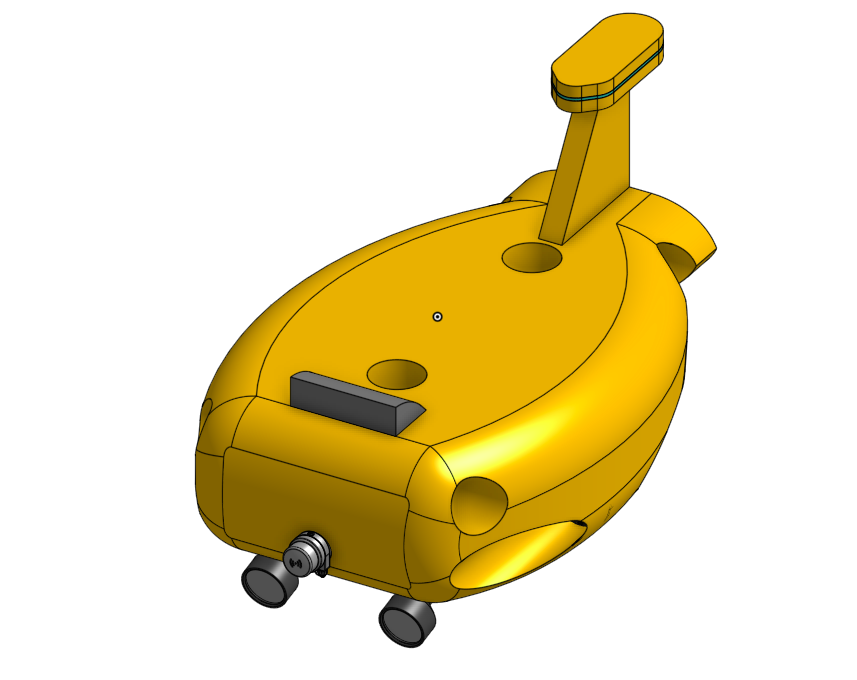
\includegraphics[trim = 0 20 0 50, clip, width=0.4\textwidth]{turbot-fish-01modi.png}
        %\caption{.}
    \end{figure}
%*----------- notes
    \note[item]{Notes can help you to remember important information. Turn on the notes option.}
\end{frame}
%-
%*----------- SLIDE -------------------------------------------------------------
\begin{frame}[t]{Objetivos}
    Objetivo Geral
    \newline
    Desenvolver um modelo de veículo submarino para a navegação em águas rasas.
    \newline

    Objetivos Específicos
    \begin{itemize}
        \item Realizar o estudo do estado da arte
        \item Realizar o desing da estrutura do submarino
        \item Realizae simuolações (CFD,ROS)
        \item Desenvolver o planejamento dos experimentos
        \item Desenvolver artigos científicos
    \end{itemize}
   

%*----------- notes
    \note[item]{Notes can help you to remember important information. Turn on the notes option.}
\end{frame}
%-
%*----------- SLIDE -------------------------------------------------------------
\begin{frame}[c]{Metodologia }
    %\transboxin[duration=1,direction=30]
        \begin{figure}
        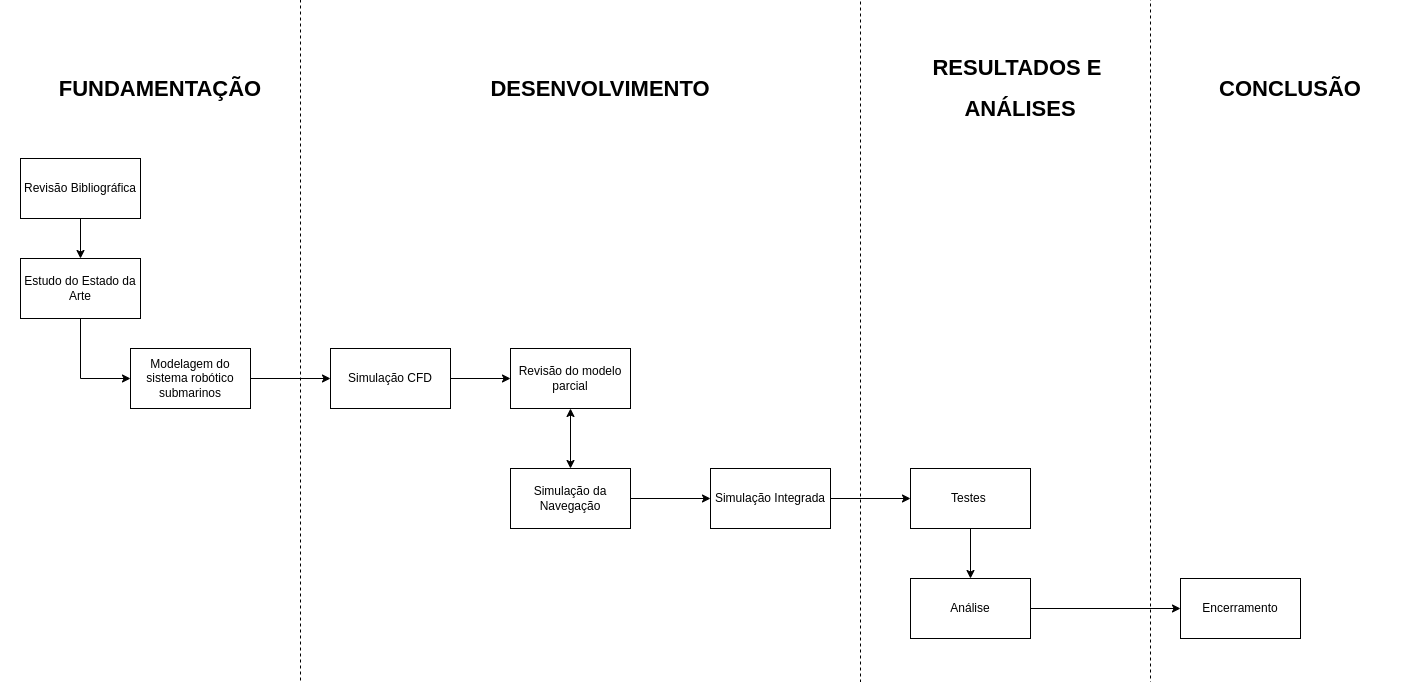
\includegraphics[width=.8\textwidth]{metodologiamodi.png}
    \end{figure}
%*----------- notes
    \note[item]{Notes can help you to remember important information. Turn on the notes option.}
\end{frame}
%-
%*----------- SLIDE -------------------------------------------------------------
\begin{frame}[t]{Método BiLi}
    %\bfseries{Ciclo Ingênuo} 
    Ciclo Ingênuo 
    \newline
        Foram pesquisados 10 ".bib" para chegar no resultado 
    \newline
        Palavras chaves: underwater vehicle,underwater robotics,cfd modeling,cfd simulation, OpenFOAM
    \newline
        Artigos encontrados: 633
    \newline
        String gereada: "underwater vehicle" OR "autonomous underwater" OR "operated vehicle" OR
        "remotely operated" OR "robotic vehicle" OR "underwater robot") AND ("computational fluid" OR "fluid dynamic") 
        AND ("control system" OR "fluid dynamics")
    \newline
    Ciclo Otmizado
    \newline
        Utilização do litserach para otimização da strin
    \newline
        Artigos encontrados: 733
    \newline
        Filtragem do RevTools: 357 artigos

%*----------- notes
    \note[item]{Notes can help you to remember important information. Turn on the notes option.}
\end{frame}
%-
%*----------- SLIDE -------------------------------------------------------------
\begin{frame}[t]{Ciclo Ingênuo X Ciclo Otmizado}
    \transboxout[duration=0.5]
    \framesubtitle{Taxa de crescimento anual de artigos científicos}
    
    \begin{columns}
        \column{.4\textwidth}
        \newline  
            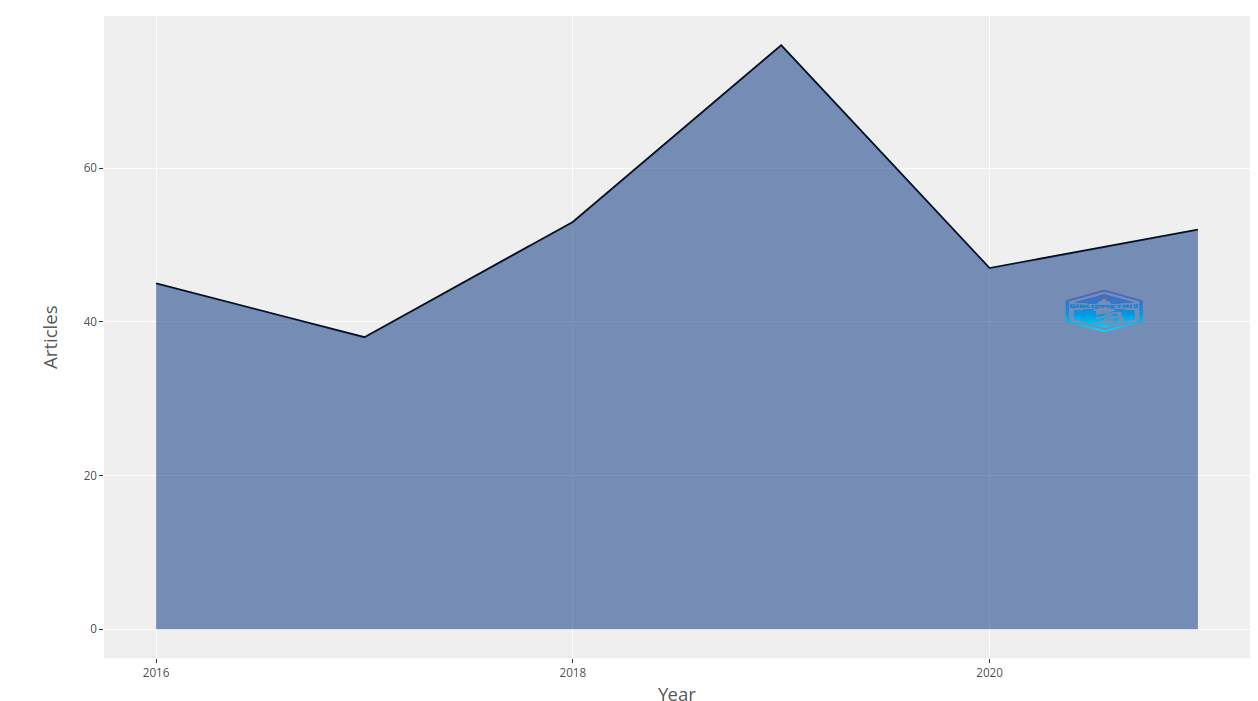
\includegraphics[height = 4cm, width=1.2\textwidth]{produçãoanual1.png}
        \column{.4\textwidth}
        \newline  
         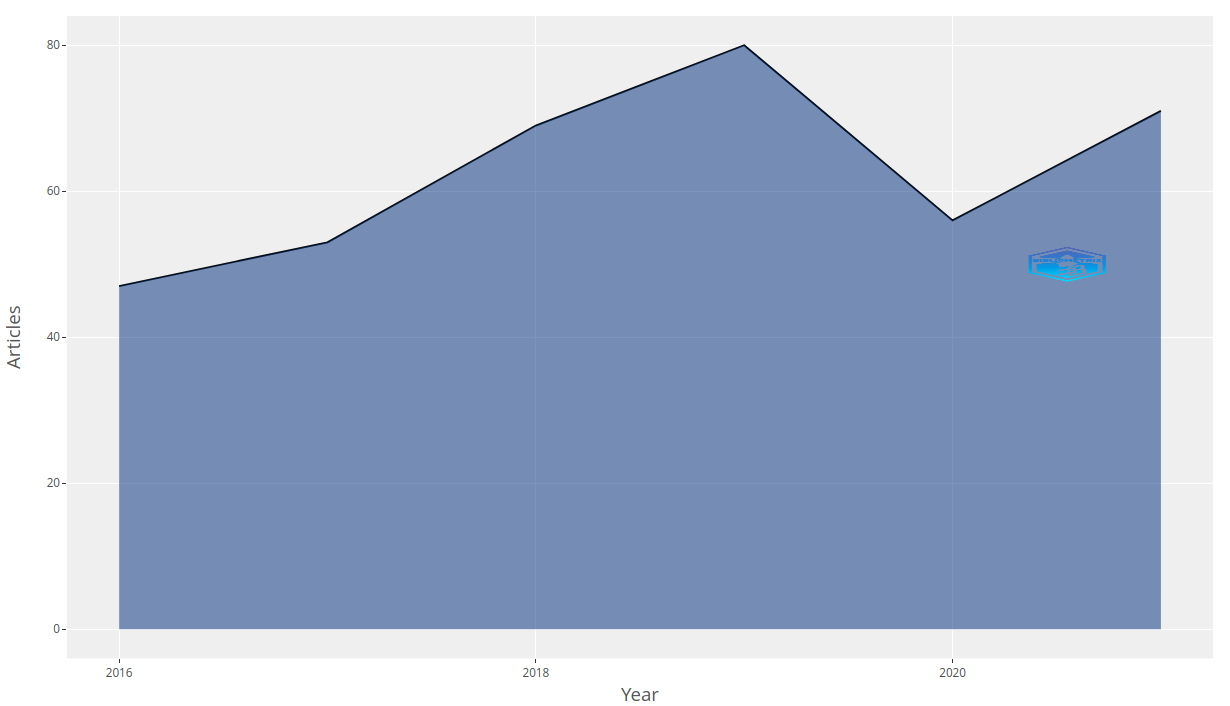
\includegraphics[height = 4cm, width=1.2\textwidth]{producaanual2.png}
    \end{columns}
    
    \begin{columns}
        \column{.4\textwidth}
        \newline  
        Taxa de crescimento: 2.93\%
        \column{.4\textwidth}
        \newline
         Taxa de crescimento: 8.6\%
    \end{columns}
 %*----------- notes
    \note[item]{Notes can help you to remember important information. Turn on the notes option.}
\end{frame}
%-
%*----------- SLIDE -------------------------------------------------------------
\begin{frame}[t]{Ciclo Ingênuo X Ciclo Otmizado}
    \transboxout[duration=0.5]
    \framesubtitle{Rede de co-citação}
    
    \begin{columns}
        \column{.4\textwidth}
        \newline  
            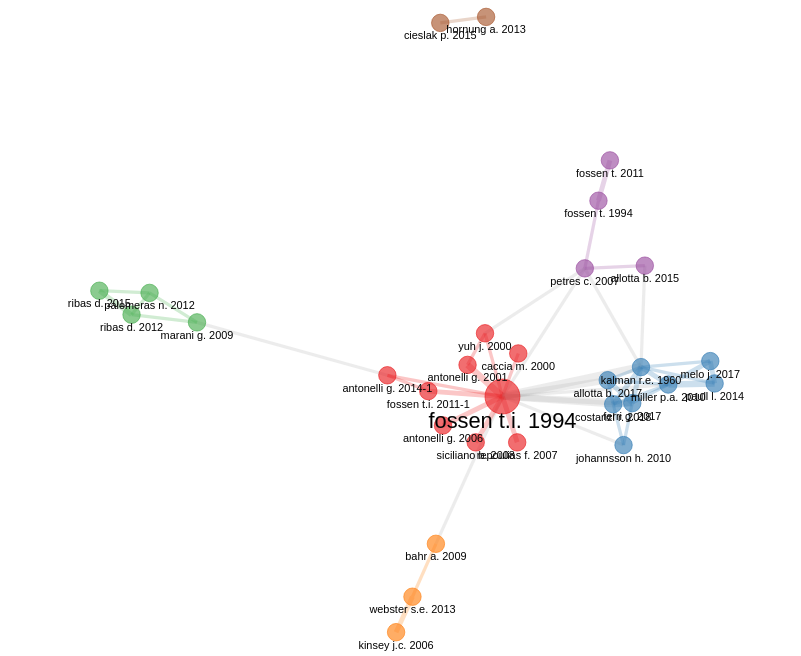
\includegraphics[height = 5cm, width=1.2\textwidth]{cocitação1.png}
        \column{.4\textwidth}
        \newline  
         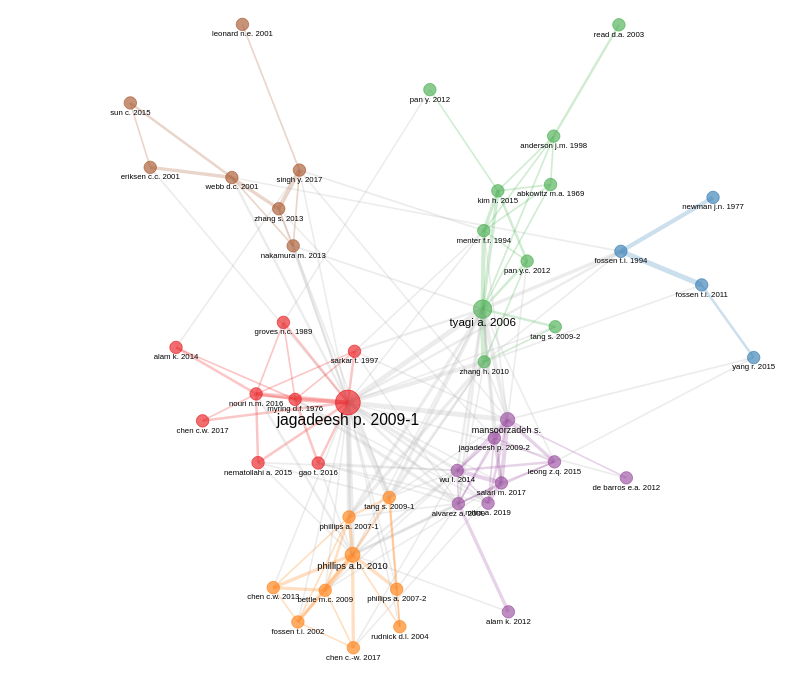
\includegraphics[height = 5cm, width=1.2\textwidth]{cocitação2.png}
    \end{columns}
    
 %*----------- notes
    \note[item]{Notes can help you to remember important information. Turn on the notes option.}
\end{frame}
%-
%*----------- SLIDE -------------------------------------------------------------
\begin{frame}[t]{Ciclo Ingênuo X Ciclo Otmizado}
    \transboxout[duration=0.5]
    \framesubtitle{Mapa de palavras}
    
    \begin{columns}
        \column{.4\textwidth}
        \newline  
            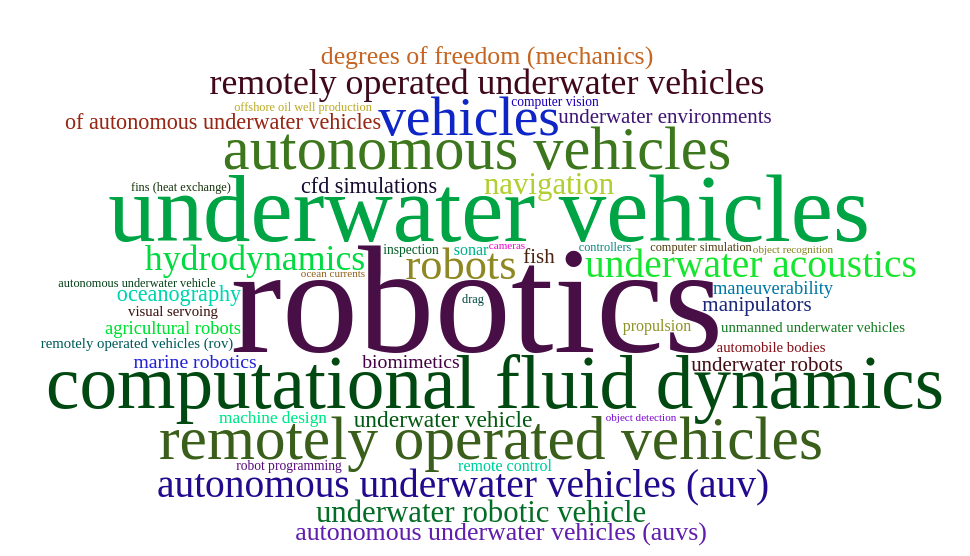
\includegraphics[height = 4cm, width=1.2\textwidth]{mapadepalavras1.png}
        \column{.4\textwidth}
        \newline  
         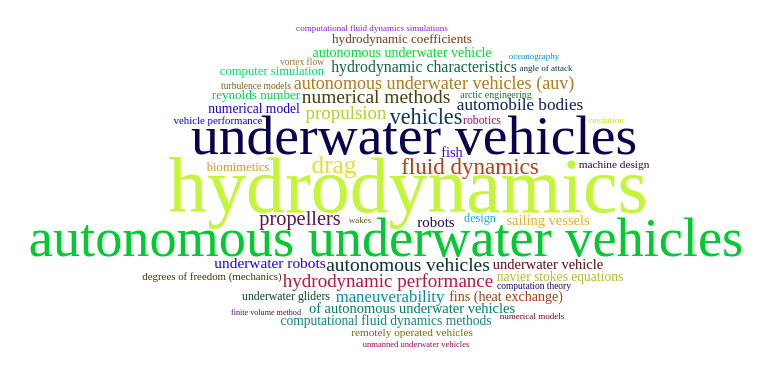
\includegraphics[height = 4cm, width=1.2\textwidth]{mapadepalavras2.png}
    \end{columns}
    
 %*----------- notes
    \note[item]{Notes can help you to remember important information. Turn on the notes option.}
\end{frame}
%-
%*----------- SLIDE -------------------------------------------------------------
\begin{frame}[c]{Cronograma}
    %\transboxin[duration=1,direction=30]
        \begin{figure}
        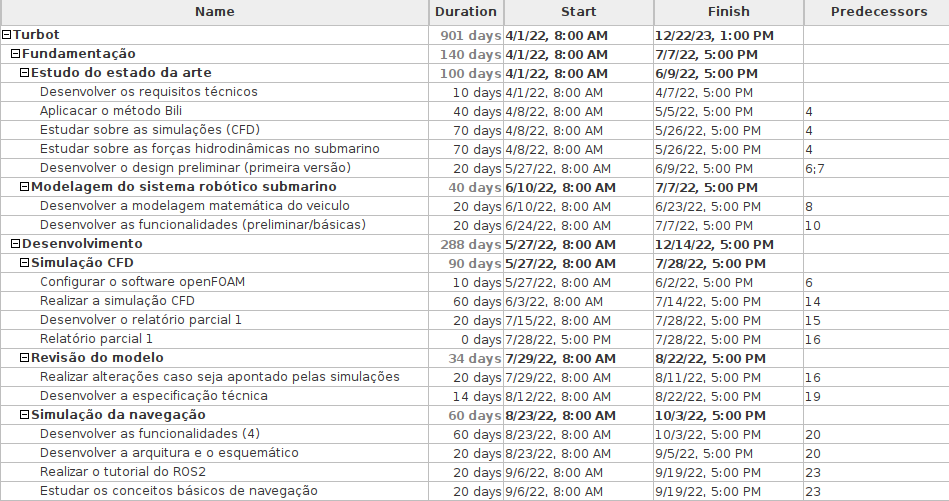
\includegraphics[width=.9\textwidth]{cronograma1.png}
    \end{figure}
%*----------- notes
    \note[item]{Notes can help you to remember important information. Turn on the notes option.}
\end{frame}
%-
%*----------- SLIDE -------------------------------------------------------------
\begin{frame}[c]{Cronograma}
    %\transboxin[duration=1,direction=30]
        \begin{figure}
        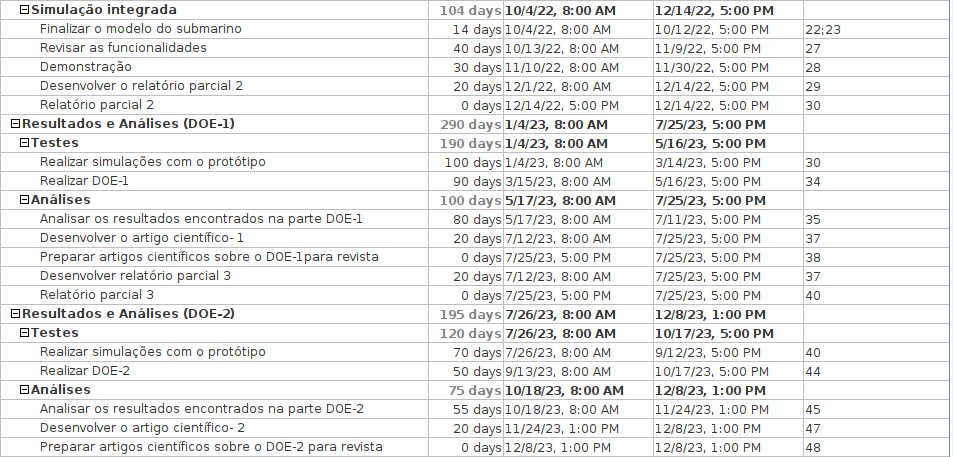
\includegraphics[width=.9\textwidth]{cronograma2.png}
    \end{figure}
%*----------- notes
    \note[item]{Notes can help you to remember important information. Turn on the notes option.}
\end{frame}
%-
%*----------- SLIDE -------------------------------------------------------------
\begin{frame}[c]{Cronograma}
    %\transboxin[duration=1,direction=30]
        \begin{figure}
        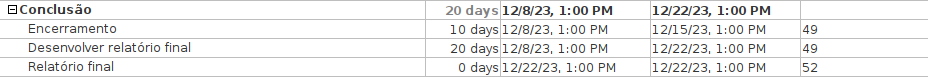
\includegraphics[width=1\textwidth]{cronograma3.png}
    \end{figure}
%*----------- notes
    \note[item]{Notes can help you to remember important information. Turn on the notes option.}
\end{frame}
%-
%*----------- SLIDE -------------------------------------------------------------
\begin{frame}[c]{A tropa dos quatro incríveis}
    %\transboxin[duration=1,direction=30]
    A simulação deverá ser desenvolvida com 4 unidades Darwin-OP, comumente esta unidade é utilizada para desafios em competições de robótica.
    \newline

    A tropa será composta por 4 Darwin-OP, e deverá realizar duas missões:
    \begin{itemize}
        \item marchar em forma unida em linha;
        \item realizar corrida de revezamento.
    \end{itemize}

    \begin{figure}
        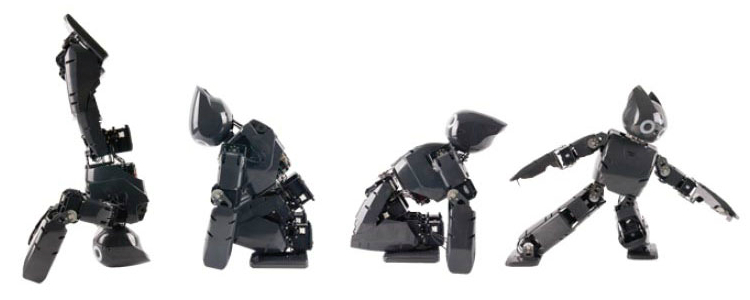
\includegraphics[trim = 0 20 0 50, clip, width=0.8\textwidth]{darwin-op-sequencia}
        %\caption{.}
    \end{figure}
%*----------- notes
    \note[item]{Notes can help you to remember important information. Turn on the notes option.}
\end{frame}
%-
%*----------- SLIDE -------------------------------------------------------------
\begin{frame}[t]{Algumas regras}
    \begin{itemize}
        \item A marcha deverá ser realizada diante de um percurso de 2 metros.
        \item A marcha e a corrida de revezamento deverão serem realizadas numa pista de corrida;
        \item A corrida deverá ser realizada numa pista de 8 metros;
        \item Cada Darwin-OP deverá percorrer 2 metros para realizar o revezamento;
        \item A região de revezamento deverá ser uma área de até 0.4 metros;
        \item O conceito para o revezamento será o de alinhar-se os dois Darwin-OP durante até 15 segundos a uma distância de no máximo 0.2 metros entre ambos, ou seja será considerado passagem de bastão quando os dois Darwin-OP passarem 15 segundos com movimentos sincronizados a uma distância máxima de 0.2 metros dentro da região de revezamento;
        \item A pista de corrida deverá ser considerada analogamente a uma pista real;
        \item A lateral da pista deverá ter lados de 2 metros;
        \item Considerar sempre os critérios de uma corrida de revezamento.
    \end{itemize}
   
    % \begin{columns}[t]
    %     \column{.45\textwidth}
    %         detalhar sistemas em subconjuntos\\
    %         listar possíveis modos de falhas\\
    %         analisar cada modo de falha, juntamente com suas possíveis causas e sintomas
    %     \column{.45\textwidth}
    %         estimar os efeitos de cada modo de falhas\\
    %         estimar a criticidade de cada efeito\\
    %         identificar ações para minimizar falhas
    % \end{columns}
%*----------- notes
    \note[item]{Notes can help you to remember important information. Turn on the notes option.}
\end{frame}
%-
%*----------- SLIDE -------------------------------------------------------------
\begin{frame}[c]{A pista}
    \begin{figure}
        %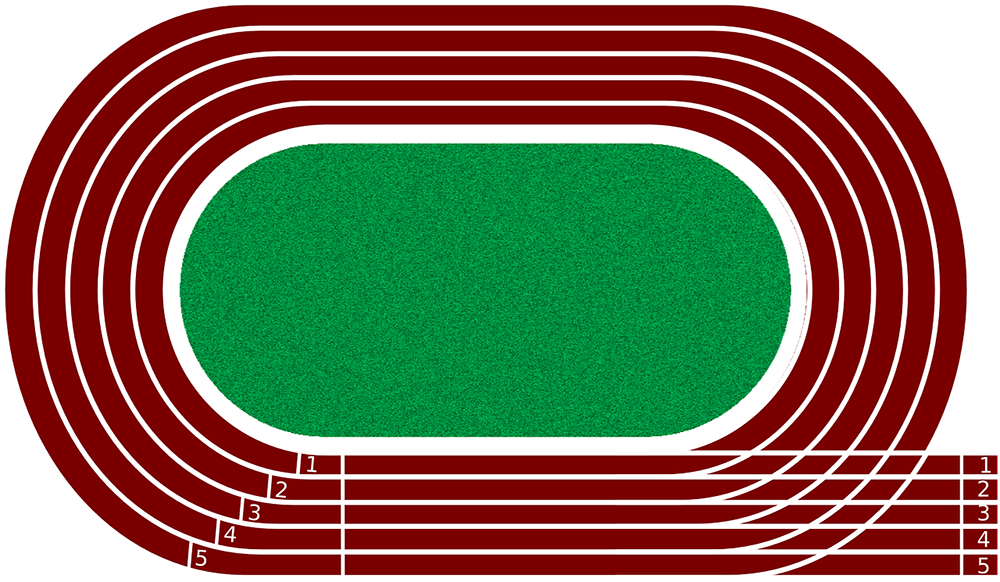
\includegraphics[width=0.7\textwidth]{pista_corrida}
       
        \roundpic[xshift=0cm,yshift=0cm]{3cm}{7cm}{pista_corrida}
          
        \caption{Formato de um pista de corrida.\cite{agostini2007}}
    \end{figure}
%*----------- notes
    \note[item]{Notes can help you to remember important information. Turn on the notes option.}
\end{frame}
%-
%*----------- SLIDE -------------------------------------------------------------
\begin{frame}[t]{As lideranças das equipes dos Novos Talentos}
    \vspace{0.5cm}
    \begin{columns}
        \column{.01\textwidth}
        \column{.7\textwidth}
            \begin{itemize}
                \item equipe \tikznode{cmark}{RAJA} será liderada por Aziel Freitas
                \item equipe \Circled[outer color=mracula8, inner ysep=8pt]{BORG} será liderada por Mateus Cerqueira.
                \item equipe \Circled[outer color=mracula7, inner ysep=8pt]{BORG} será liderada por Mateus Cerqueira.
                \item equipe \Circled[outer color=mracula9, inner ysep=8pt]{jerotimon} será liderada por Mateus Cerqueira.
                \item equipe TIMON-HM será liderada por Leonardo Lima.
            \end{itemize}
        \column{.29\textwidth}
            
\includegraphics[width=.9\textwidth, trim={10cm 0 10cm 0},clip]{equipe}
    \end{columns}
    \vspace{1cm}
    
    \emph{Para este desafio não será cobrado o relatório técnico, porém o acompanhamento deverá seguir o mesmo ritmo dos desafios anteriores.}

    %add circle on word
    \begin{tikzpicture}[remember picture,overlay]
        \draw[mracula5,very thick] (cmark) circle[x radius=8mm,y radius=4mm]; 
    \end{tikzpicture}
%*----------- notes
    \note[item]{Notes can help you to remember important information. Turn on the notes option.}
\end{frame}
%-
%*----------- SLIDE -------------------------------------------------------------
\begin{frame}[t]{O progresso das equipes}
    Um dos indicadores para o acompanhamento das equipes será o percentual de conclusão geral da equipe.
    O planejamento das atividades deverá seguir a metodologia aplicada no desenvolvimento de projetos de robótica.
    \newline
    %\vspace{0.5cm}
    \begin{table}[ht!]
    \centering
        \caption{PERCENTUAL DE CONCLUSÃO POR EQUIPE}
        \begin{tabular}{|l|c|c|c|c|} \hline
            \textbf{EQUIPE}&\textbf{04/05}&\textbf{11/05}&\textbf{18/05}&\textbf{25/05}\\ \hline
            RAJA & 17\% &32\% & &  \\ \hline
            BORG & 0\% &41\% & &  \\ \hline
            TIMON-HM & 5\% &47\% & &  \\ \hline
        \end{tabular}
    \end{table}
%*----------- notes
    \note[item]{Notes can help you to remember important information. Turn on the notes option.}
\end{frame}
%-
%*----------- SLIDE -------------------------------------------------------------
\begin{frame}[t]{O progresso das equipes}
    Um dos indicadores para o acompanhamento das equipes será o percentual de conclusão geral da equipe.
    O planejamento das atividades deverá seguir a metodologia aplicada no desenvolvimento de projetos de robótica.
    \newline
    %\vspace{0.5cm}
    % \begin{table}[ht!]
    % \centering
    %     \caption{PERCENTUAL DE CONCLUSÃO POR EQUIPE}
    %     \begin{tabular}{|l|c|c|c|c|} \hline
    %         \textbf{EQUIPE}&\textbf{04/05}&\textbf{11/05}&\textbf{18/05}&\textbf{25/05}\\ \hline
    %         RAJA & 17\% &32\% & &  \\ \hline
    %         BORG & 0\% &41\% & &  \\ \hline
    %         TIMON-HM & 5\% &47\% & &  \\ \hline
    %     \end{tabular}
    % \end{table}
%*----------- notes
    \note[item]{Notes can help you to remember important information. Turn on the notes option.}
\end{frame}
%-
%*----------- SLIDE -------------------------------------------------------------
\begin{frame}[t]{O progresso das equipes}
    Um dos indicadores para o acompanhamento das equipes será o percentual de conclusão geral da equipe.
    O planejamento das atividades deverá seguir a metodologia aplicada no desenvolvimento de projetos de robótica.
    \newline
    %\vspace{0.5cm}
    % \begin{table}[ht!]
    % \centering
    %     \caption{PERCENTUAL DE CONCLUSÃO POR EQUIPE}
    %     \begin{tabular}{|l|c|c|c|c|} \hline
    %         \textbf{EQUIPE}&\textbf{04/05}&\textbf{11/05}&\textbf{18/05}&\textbf{25/05}\\ \hline
    %         RAJA & 17\% &32\% & &  \\ \hline
    %         BORG & 0\% &41\% & &  \\ \hline
    %         TIMON-HM & 5\% &47\% & &  \\ \hline
    %     \end{tabular}
    % \end{table}
    
    \url{https://braziliansinrobotics.com/}
%*----------- notes
    \note[item]{Notes can help you to remember important information. Turn on the notes option.}
\end{frame}
%-
%*----------- SLIDE -------------------------------------------------------------
\begin{frame}[c]{}
    \begin{center}
        \Wider{%
        \begin{shaded}
        \begin{center}
            \vspace*{0.8cm}
            \resizebox{!}{1cm}{%
               % \color{bg} O objetivo é ter um objetivo.
                \begin{tabular}{ccc}
                    \textbf{Projetos}   
                  \end{tabular}
            }%
        \end{center}
        \end{shaded}
        }%
    \end{center}
%*----------- notes
    \note[item]{Notes can help you to remember important information. Turn on the notes option.}
\end{frame}
%-
%*----------- SLIDE -------------------------------------------------------------
\begin{frame}[t]{FlatFish@ROS}
    Atualizar o framework utilizado no protótipo do FlatFish, migrando para o ROS.
    
    \begin{center}
    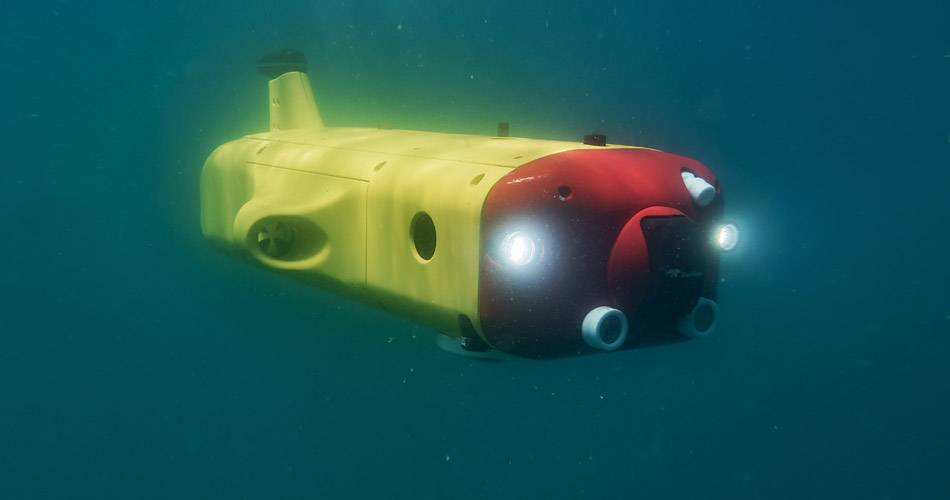
\includegraphics[width=0.5\textwidth]{flatfish.jpg}
    \end{center}
    
    
            
\end{frame}
%*----------- SLIDE -------------------------------------------------------------
\begin{frame}[t]{FlatFish@ROS}
    \framesubtitle{Desenvolvido}
    \begin{itemize}
        \item Elaborado o cronograma do projeto
        \item Estudo ROS
        \item Conexão do computador central FlatFISH
        \item Ajustes na NUC
    \end{itemize}    
%*----------- notes
    \note[item]{Notes can help you to remember important information. Turn on the notes option.}
\end{frame}
%-
%*----------- SLIDE -------------------------------------------------------------
\begin{frame}[t]{FlatFish@ROS}
    \framesubtitle{Próximos passos}
    \begin{itemize}
        \item Listar as funcionalidades para desenvolvimento da montagem do sistema robótico submarino
        \item Simulação no openFOAM
        \item Simulação no ROS
        \item Desenvolvimento de 4 artigos: 
        \begin{itemize}
            \item[] 2022- SOTA e Simulação OpenFOAM
            \item[] 2023- DOE OpenFOAM e ROS 
        \end{itemize}  
        
    \end{itemize}    
%*----------- notes
    \note[item]{Notes can help you to remember important information. Turn on the notes option.}
\end{frame}
%-


\begin{frame}[t]{Pirabots}
     Implmentar ações autônomas em ROVs: BlueROV e BirROV.
      
   
    \begin{columns}
        \column{.45\linewidth}
    \begin{center}

        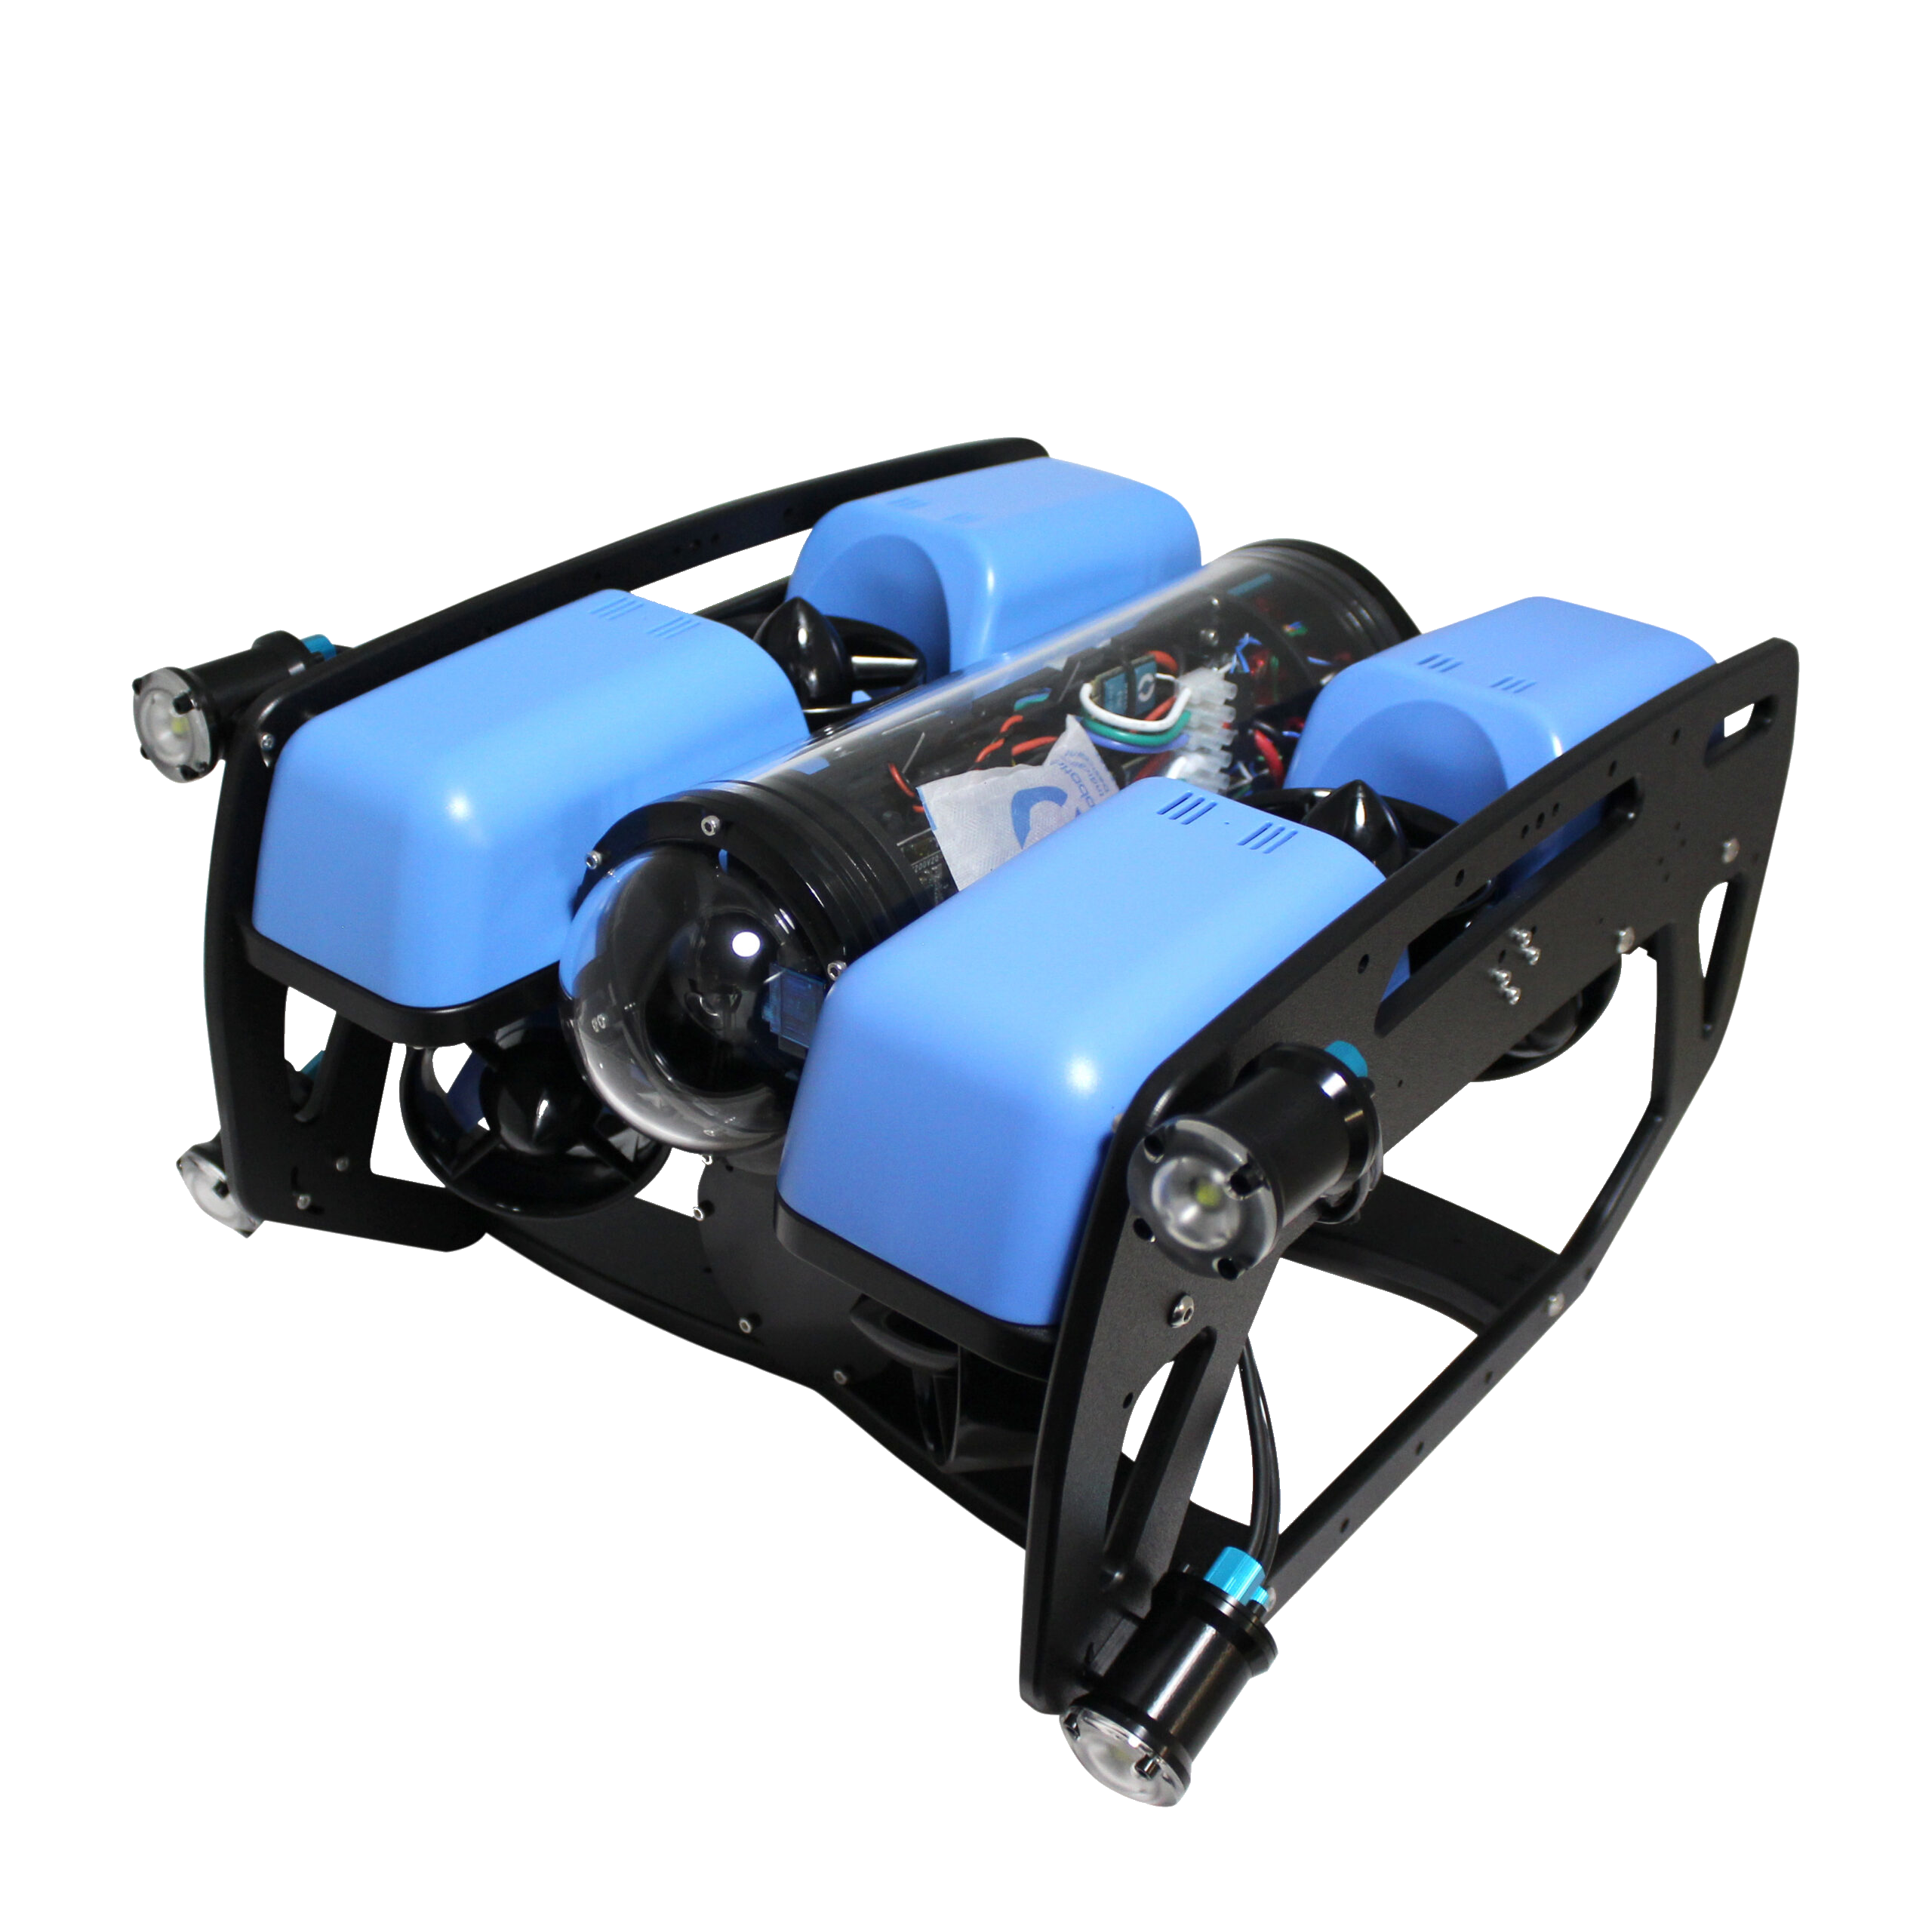
\includegraphics[width=0.8\textwidth]{bluerov.png}

    \end{center}

    \column{.45\linewidth}
    \vspace*{0.3cm}
    \begin{center}

        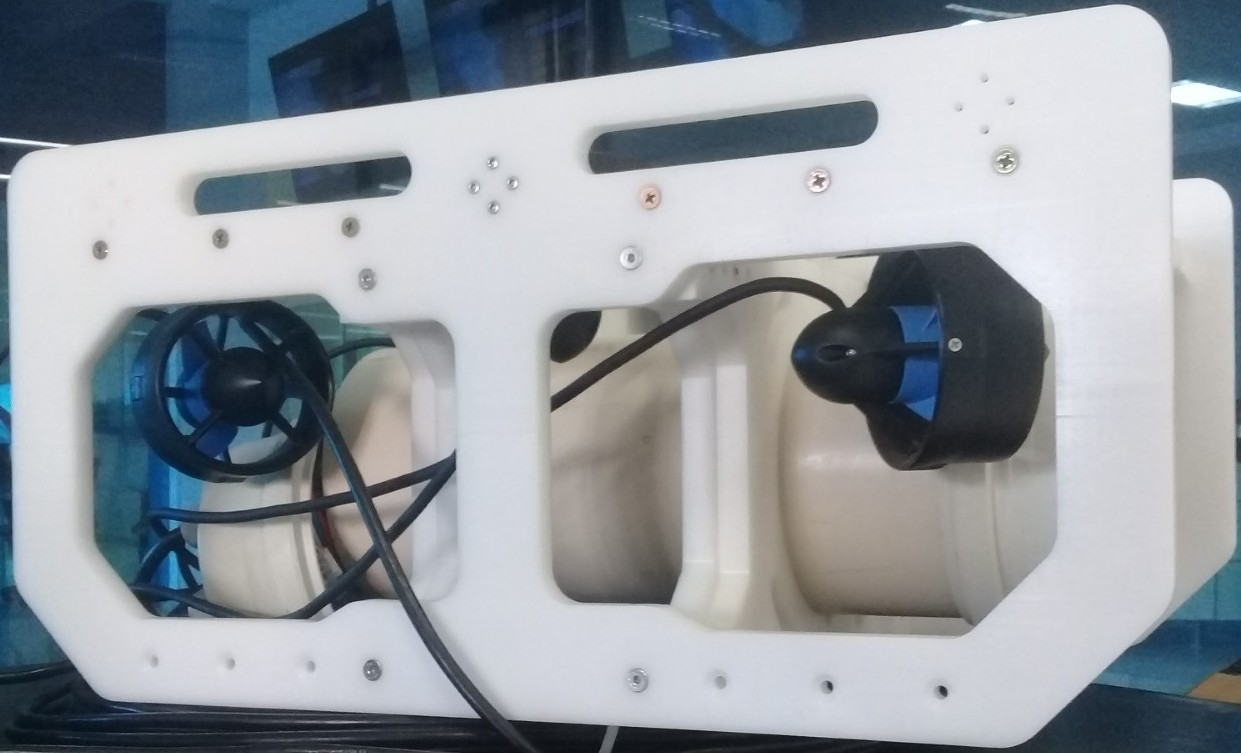
\includegraphics[width=0.8\textwidth]{bir_rov.jpg}

    \end{center}

\end{columns}

\end{frame}
%*----------- SLIDE -------------------------------------------------------------
\begin{frame}[t]{Pirabots}
    \framesubtitle{Desenvolvido}
    \begin{itemize}
        \item Elaborado o cronograma do projeto
        \item Estudo ROS
        \item Desenvlvimento do SOTA sobre ROV semi-autônomo
        \item Simulações no tanque do CIMATEC
    \end{itemize}    
%*----------- notes
    \note[item]{Notes can help you to remember important information. Turn on the notes option.}
\end{frame}
%-
%*----------- SLIDE -------------------------------------------------------------
\begin{frame}[t]{Pirabots}
    \framesubtitle{Próximos passos}
    \begin{itemize}
        \item Listar as funcionalidades para desenvolvimento da montagem do sistema robótico submarino
        \item Simulação no openFOAM
        \item Simulação no ROS
        \item Desenvolvimento de 4 artigos: 
        \begin{itemize}
            \item[] 2022- SOTA e Simulação OpenFOAM
            \item[] 2023- DOE OpenFOAM e ROS 
        \end{itemize}  
        
    \end{itemize}    
%*----------- notes
    \note[item]{Notes can help you to remember important information. Turn on the notes option.}
\end{frame}
%-

%*----------- SLIDE -------------------------------------------------------------
\begin{frame}[c]{turBOT}
    Desenvolver um veículo submarino autônomo para atuar em águas rasas para fins exploratórios,
    o veículo em desenvolvimento terá capacidade de identificar algumas anomalias ou padrões construídos
    e disponibilizará para os pesquisadores, apresenta uma dimensão menor do que os veículos comerciais.
    \begin{figure}
        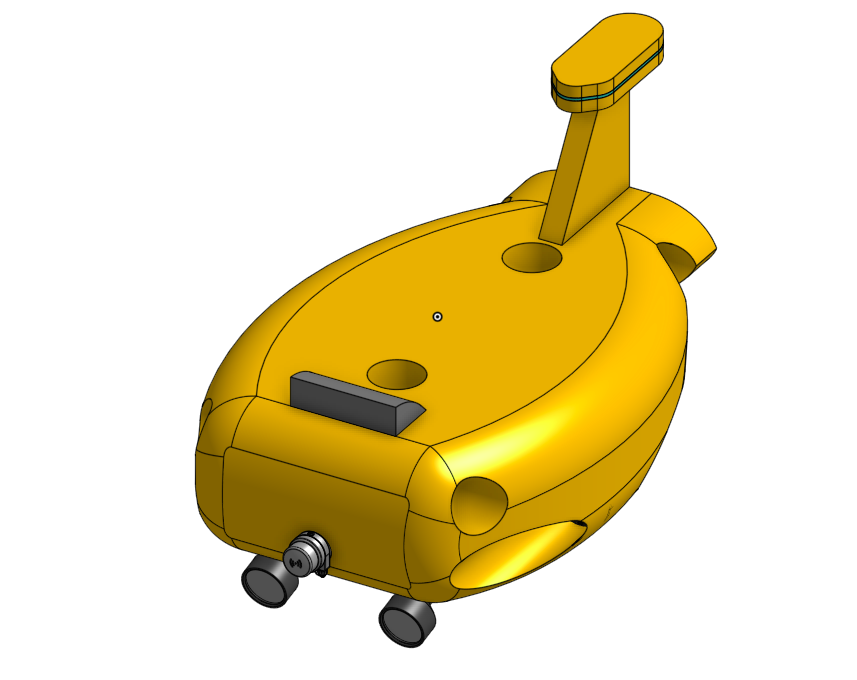
\includegraphics[width=.4\textwidth]{turbot-fish-01modi.png}
    \end{figure}
    
%*----------- notes
    \note[item]{Notes can help you to remember important information. Turn on the notes option.}
\end{frame}
%-
%*----------- SLIDE -------------------------------------------------------------
\begin{frame}[c]{turBOT }
    \framesubtitle{Metodologia}
    %\transboxin[duration=1,direction=30]
        \begin{figure}
        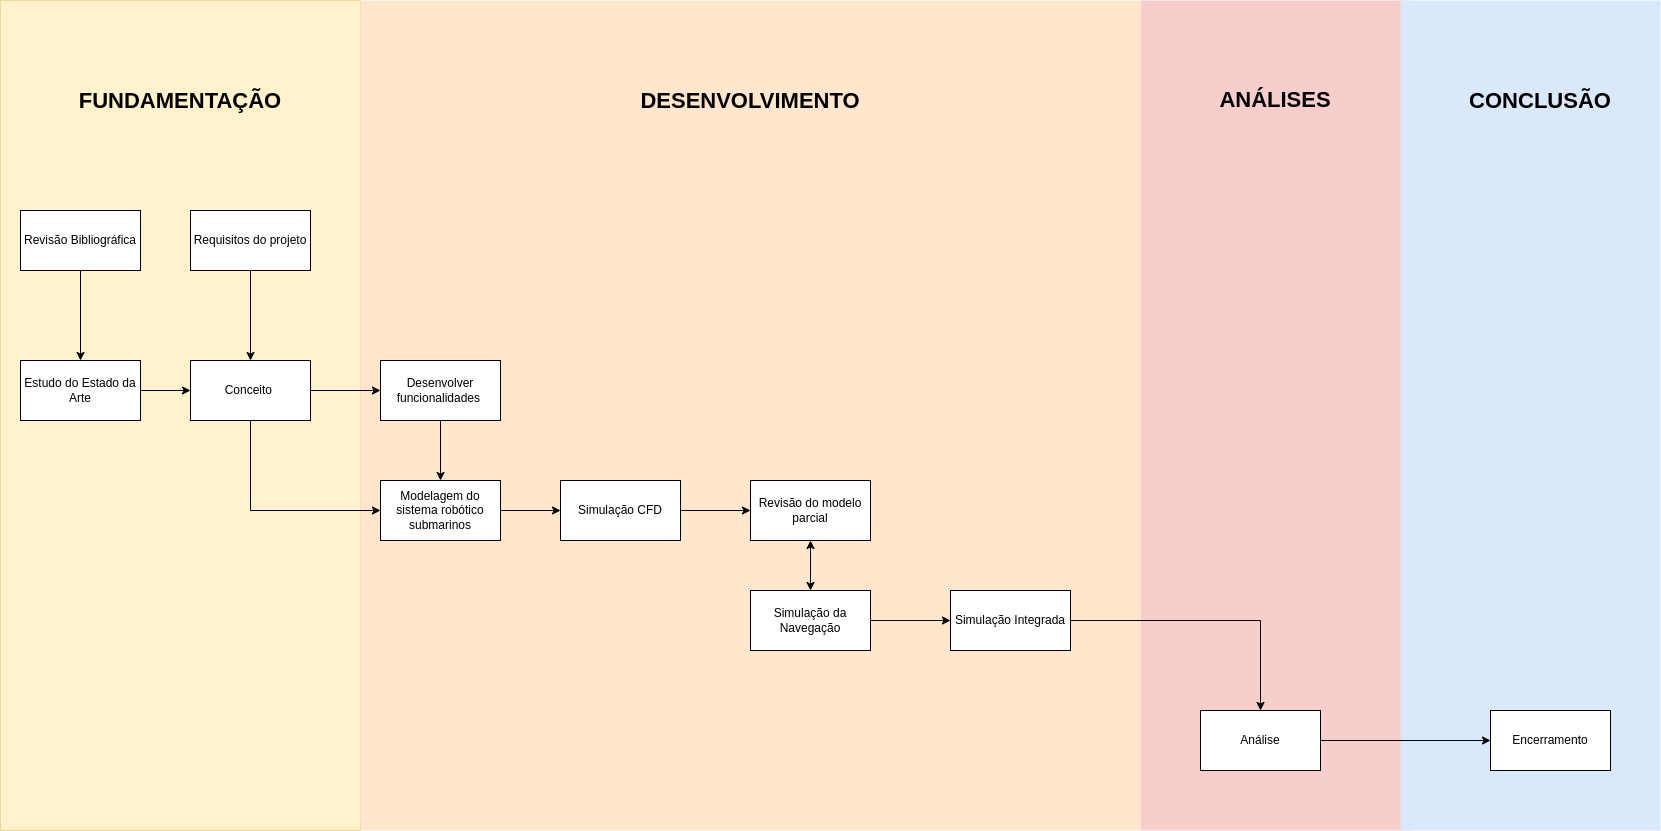
\includegraphics[width=.9\textwidth]{metodolodia3.png}
    \end{figure}
%*----------- notes
    \note[item]{Notes can help you to remember important information. Turn on the notes option.}
\end{frame}
%-
%*----------- SLIDE -------------------------------------------------------------
\begin{frame}[t]{turBOT}
    \framesubtitle{Desenvolvido}
    \begin{itemize}
        \item Elaborado o cronograma do projeto
        \item Realizado o método BiLi
        \item Estudos sobre linguagens de programação C++, Python e R
        \item Estudo ROS e openFOAM
        \item Estudo sobre CFD (Fluidodinâmica computacional)v
    \end{itemize}    
%*----------- notes
    \note[item]{Notes can help you to remember important information. Turn on the notes option.}
\end{frame}
%-
%*----------- SLIDE -------------------------------------------------------------
\begin{frame}[t]{turBOT}
    \framesubtitle{Próximos passos}
    \begin{itemize}
        \item Listar as funcionalidades para desenvolvimento da montagem do sistema robótico submarino
        \item Simulação no openFOAM
        \item Simulação no ROS
        \item Desenvolvimento de 4 artigos: 
        \begin{itemize}
            \item[] 2022- SOTA e Simulação OpenFOAM
            \item[] 2023- DOE OpenFOAM e ROS 
        \end{itemize}  
        
    \end{itemize}    
%*----------- notes
    \note[item]{Notes can help you to remember important information. Turn on the notes option.}
\end{frame}
%-
%----------------------------------------------------SLIDE------------------
 \begin{frame}[t, allowframebreaks]{References}
 %\frametitle{References}
%\begin{frame}{Reference}
    %\transboxin[duration=1,direction=30]

    % \begin{bibunit}[plain]
    % \cite{guangyi2018research}.
    % %\cite{kanakia2012}
    % %\cite{agostini2007}
    % %\cite{azuma1997survey}
    % \cite{Buss2005}
  
    % \putbib
    % \end{bibunit}
  
    %\bibliographystyle{IEEEtran}
    %\bibliographystyle{IEEEtranS}
    %\bibliographystyle{IEEEbib}
    \bibliographystyle{abntex2-alf}
    %\bibliographystyle{abntex2-num}
    %\bibliographystyle{abnt-alf}
    \bibliography{bibliography} 
    %\putbib

%*----------- notes
    %\note[item]{Notes can help you to remember important information. Turn on the notes option.}
\end{frame}
%
%-
%*----------- SLIDE-BACKUP ------------------------------------------------------
% \backupbegin
% %
% \begin{frame}{Backup}
%     Test
% %*----------- notes-------------------------------
% \note{Notes can help you to remember important information. Turn on the notes option.}
% \end{frame}
% %-
% \backupend
% %-
%*----------- QUESTIONS ---------------------------------------------------------
\begin{frame}[c,plain]
    \lastpage{
        \begin{center}   
            {\usebeamerfont{title} Questions?}\\[3ex] 
            %\hspace{1.5cm} 
            marco.a.reis@google.com
        \end{center}
    }
    
    %*----------- notes---------------------------------
    \note[item]{Notes can help you to remember important information. Turn on the notes option.}
\end{frame}
%*-------------------------------------------------------------------------------
\end{document}